\chapter{Mike Kessner: Private Equity, Team Selling, and the Long Game}

This chapter follows a School of Hard Knocks interview with Mike Kessner from \emph{10 Questions with a Millionaire}, curated for this book by LazyingArt LLC through Video2Book. There are no validated blackboard screenshots or visible equations for this lecture. The serious structure is therefore not a physics derivation but a commercial one: claims, numbers, reversals, and mechanisms by which a career becomes durable, a sales organization compounds knowledge, and a person can rebuild if the balance sheet goes to zero.

\section{The Private-Equity Answer Comes Back}

The interview begins by returning to a previous public moment. In an earlier School of Hard Knocks street interview, Mike was asked what industry was best for getting wealthy, and his answer was private equity. The host recalls that the clip went far beyond a normal interview answer, reaching well over two million views.

We can keep that as the first quantitative anchor:
\begin{equation}
V_{\text{clip}} > 2{,}000{,}000,
\end{equation}
where \(V_{\text{clip}}\) is the recalled view count of the earlier private-equity answer.

The point is not that two million views proves the answer correct. The point is that the interview begins with a claim that already has a public life. Mike then adds a family update: his son left consulting for a large private-equity firm, and his son-in-law left investment banking to start a private-equity firm. He does not present this as something he orchestrated. He calls it serendipitous. Still, it gives the earlier answer a new kind of evidence: not a theorem, but a witness.

\begin{remark}
Private equity should be treated here as an interviewed judgment, not as a universal prescription. Mike's own tone is important: he says it was his honest answer, even though his insurance friends would have preferred him to promote their industry.
\end{remark}

\section{False Starts Before the Long Path}

The interviewer then asks where Mike actually began. The answer is not a clean founder myth. Mike went to LSU thinking he might play baseball, sat on the bench, transferred to the University of Denver, and later joked that LSU became strong after he left. His first job after college was as a headhunter, but he quit after roughly a month because he disliked the cold, the early mornings, and the commute into downtown Chicago.

That early instability matters. The interview is not saying, ``choose the right industry at eighteen and everything follows.'' It is saying something less glamorous and more useful: a durable career can start with awkward fits and low grit. Mike moved through a large company, relocated to St. Louis, met his wife there, and later returned home partly because his mother was widowed. That return brought him into insurance.

The time scale is the first real structure:
\begin{align}
T_{\text{insurance}} &> 30 \ \text{years},\\
T_{\text{uncertain}} &\approx 3\text{--}4 \ \text{years}.
\end{align}
The two lines belong together. Mike's insurance career lasts more than thirty years, but he says he did not know what he was doing for the first three or four. The early confusion is not edited out of the mechanism.

\subsection{Question \& Answer}

\paragraph{Question.}
How does an uncertain early career become a long-term wealth path?

\paragraph{Answer.}
In Mike's telling, the early years did not become valuable because he had already mastered the work. They became valuable because he stayed near people he judged to be authentic, good, and high-energy. The commercial mechanism begins socially: choose the room, survive the apprenticeship, and give time enough room to reveal which people and opportunities compound.

\section{The Long Game Becomes an Offer}

Mike gives his central career rule in simple language. If he stayed around authentic, high-energy people, he believed they would eventually become successful; if he stayed with them long enough, he would participate in that success. He says he played this long game for probably more than twenty-five years:
\begin{equation}
T_{\text{long game}} > 25 \ \text{years}.
\end{equation}

The payoff arrives through relationship rather than prediction. Mike met a young CEO of an insurance firm roughly five years before the interview. At first, he thought his old firm might buy that company. The old firm had grown large, with about two thousand people, and was part of a private-equity roll-up:
\begin{equation}
N_{\text{prior firm}} \approx 2{,}000.
\end{equation}
Instead of an acquisition by the old firm, Mike and his partner became friends with the younger CEO. A year later, over dinner, the younger CEO made them an offer they could not refuse. Mike describes the next three and a half years as the most enjoyable period of his insurance career, largely because he was coaching younger people and leaving a legacy.

We can write the mechanism cautiously:
\begin{equation}
\text{credible people}+\text{time}+\text{fit}
\longrightarrow
\text{opportunity flow}.
\end{equation}
This is not a law of business. It is the structure Mike narrates: relationships accumulate value before the offer is visible.

\begin{figure}
\centering
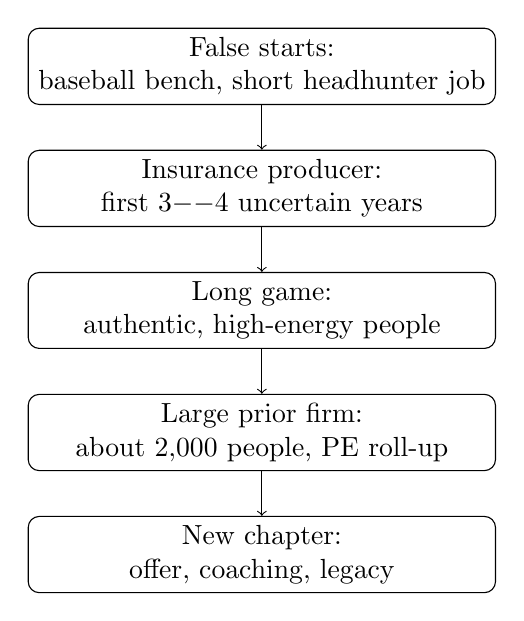
\begin{tikzpicture}[x=1cm,y=1cm]
\node[draw, rounded corners, align=center, text width=5.7cm] (a) at (0,0) {False starts:\\ baseball bench, short headhunter job};
\node[draw, rounded corners, align=center, text width=5.7cm] (b) at (0,-1.55) {Insurance producer:\\ first \(3\text{--}4\) uncertain years};
\node[draw, rounded corners, align=center, text width=5.7cm] (c) at (0,-3.1) {Long game:\\ authentic, high-energy people};
\node[draw, rounded corners, align=center, text width=5.7cm] (d) at (0,-4.65) {Large prior firm:\\ about \(2{,}000\) people, PE roll-up};
\node[draw, rounded corners, align=center, text width=5.7cm] (e) at (0,-6.2) {New chapter:\\ offer, coaching, legacy};
\draw[->] (a) -- (b);
\draw[->] (b) -- (c);
\draw[->] (c) -- (d);
\draw[->] (d) -- (e);
\end{tikzpicture}
\caption{A transcript-grounded career compounding ladder. The figure reconstructs the spoken sequence; no validated board diagram exists for this lecture.}
\end{figure}

\section{Luck, Timing, and Memory}

The next question asks for Mike's best and worst financial decisions. The answers are valuable because they separate return, timing, and meaning.

His best decision may have been Nautilus. He read about the company on an airplane shortly before the pandemic, noticed its connection to fitness equipment brands, invested, and then invested more once it seemed that people stuck at home would buy exercise equipment. He calls the result pure luck.

The weaker decisions are Coinbase and the family home. Coinbase gave back much of those winnings, though he was still holding. The home is a more interesting case. Mike says his family lived there for more than twenty years and roughly broke even. Financially, that sounds poor. Personally, he says he would not trade the memories.

\begin{table}
\centering
\begin{tabular}{p{0.24\linewidth}p{0.32\linewidth}p{0.31\linewidth}}
\hline
Case & Financial reading & Nonfinancial reading \\
\hline
Nautilus & Lucky timing before and during the pandemic & Useful anecdote, not a repeatable formula \\
Coinbase & Gave back some winnings & Still held with some hope \\
Family home & Roughly broke even after \(20+\) years & Preserved family memories \\
\hline
\end{tabular}
\caption{Mike's financial examples keep return, timing, and personal value in separate columns.}
\end{table}

\subsection{Question \& Answer}

\paragraph{Question.}
Can a bad investment still be a good life decision?

\paragraph{Answer.}
In this interview, yes. The family home is named among the worst financial decisions because it apparently broke even after more than twenty years. But Mike refuses to treat the memories as worthless. The right note-taking distinction is simple: financial return belongs in one column, family value in another.

\section{Analytics, Team Selling, and Vertical Knowledge}

The interviewer then circles back to the industry question. The earlier answer was private equity. In the 2023 setting of this interview, Mike adds data science and analytics. He is careful to say he is not an expert in that industry, but he sees analytics as increasingly important for insurance. Young people can crunch data, notice what is trending, and bring those patterns to experienced operators.

That naturally leads into insurance sales. If analytics helps us see the pattern, sales tests whether we can act on it with a real client. Mike's advice is that sales should not be done from an island. It should be organized like a team sport.

The firm's structure is concrete:
\begin{align}
N_{\text{sales people}} &\approx 25,\\
N_{\text{sales teams}} &\approx 5\text{--}6,\\
N_{\text{PE specialists}} &\approx 10,\\
N_{\text{restaurant clients}} &\approx 800.
\end{align}

These numbers are not decoration. They explain the operating model. A generic producer can talk about insurance. A specialized producer can talk about the client's world. Mike names private equity, hospitality, construction, and restaurants as verticals. The restaurant team, for example, can speak from hundreds of restaurant accounts and discuss retention problems, vendors, paving, and other operating headaches.

\begin{definition}
A \emph{vertical specialization} is a sales discipline organized around the client's industry rather than around a generic product pitch. In Mike's example, the salesperson becomes more credible by knowing restaurants, hospitality, construction, or private equity well enough to recognize the client's practical problems.
\end{definition}

We can express the sales mechanism as a small update rule. Let \(C_n\) denote the credibility a producer has after \(n\) relevant client examples. Then a note-quality reconstruction is
\begin{equation}
C_{n+1}
=
C_n
+
\Delta_{\text{specificity}}
+
\Delta_{\text{trust}}.
\end{equation}
The term \(\Delta_{\text{specificity}}\) increases when the producer speaks concretely about the client's vertical. The term \(\Delta_{\text{trust}}\) increases when the client believes the producer has seen similar problems before. This is a model for the chapter, not a formula from the video, but it stays faithful to Mike's phrase: the secret sauce is learning to ``talk the talk'' rather than remaining a generalist.

\begin{figure}
\centering
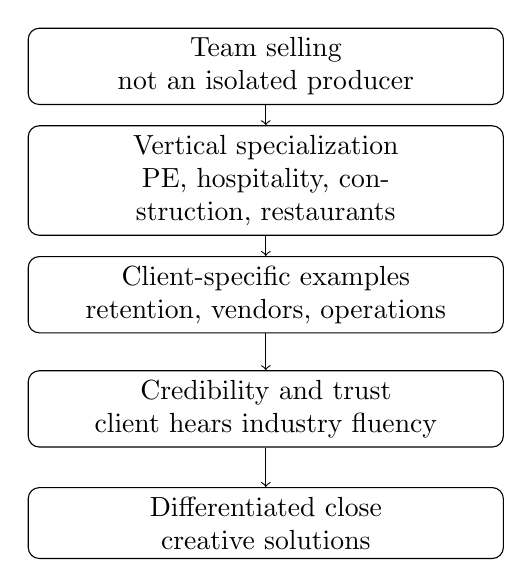
\begin{tikzpicture}[x=1cm,y=1cm]
\node[draw, rounded corners, align=center, text width=5.8cm] (a) at (0,0) {Team selling\\ not an isolated producer};
\node[draw, rounded corners, align=center, text width=5.8cm] (b) at (0,-1.45) {Vertical specialization\\ PE, hospitality, construction, restaurants};
\node[draw, rounded corners, align=center, text width=5.8cm] (c) at (0,-2.9) {Client-specific examples\\ retention, vendors, operations};
\node[draw, rounded corners, align=center, text width=5.8cm] (d) at (0,-4.35) {Credibility and trust\\ client hears industry fluency};
\node[draw, rounded corners, align=center, text width=5.8cm] (e) at (0,-5.8) {Differentiated close\\ creative solutions};
\draw[->] (a) -- (b);
\draw[->] (b) -- (c);
\draw[->] (c) -- (d);
\draw[->] (d) -- (e);
\end{tikzpicture}
\caption{The sales mechanism reconstructed from Mike's description of team selling and specialized verticals.}
\end{figure}

\section{The Operator Behind the Business}

The interview then changes register. After career, industry, and sales, the host asks about books, fatherhood, marriage, habits, mindset, and success. This is not a detour. The interview is now asking what kind of operating system keeps the business person steady.

Mike names \emph{Don't Sweat the Small Stuff} as the book that most affected him. He says it reminds him that most problems are not as large as they feel. His estimate is blunt:
\begin{equation}
p_{\text{not a big deal}} \approx 0.95.
\end{equation}
The point is not precision. The point is posture: most disturbances should not be allowed to govern the whole system.

For fatherhood, Mike emphasizes quantity of time, especially when children are young. For marriage, he gives a transition rule. If you have been a ``hammer'' at the office all day, pause before entering the house, breathe, and remember that it is time to be a partner. He also stresses affection, humor, and common interests with children.

The habits question brings the same pattern down to the morning scale. Mike says he is working harder than ever, but it does not feel like work because he is surrounded by energetic younger people. Each day begins with a triple espresso in what he calls his parlor, followed by a few minutes of meditation and gratitude toward his family, his work, Austin, and being out of Chicago weather.

The time inputs are small:
\begin{align}
t_{\text{gratitude}} &\approx 30\ \text{seconds}\text{--}5\ \text{minutes},\\
t_{\text{meditation}} &\approx 3\ \text{minutes}\quad\text{or}\quad 8\ \text{minutes}.
\end{align}

\subsection{Question \& Answer}

\paragraph{Question.}
Do habits like gratitude and meditation actually affect business performance, or are they just slogans?

\paragraph{Answer.}
Mike answers without making them grand. He says the espresso is the best part; gratitude is easy because everyone has something to be thankful for; meditation often includes thoughts about business or family. But the habit still matters because he feels good when he is done. The mechanism is not mystical. It is an opening routine that steadies attention before the workday starts.

\section{Plan, Tenacity, and the Zero-Bank-Account Test}

The interviewer next asks what mindset change people need in order to become multimillionaires. Mike answers with two pieces: actually make a plan, and then have the tenacity to execute it. Many people, he says, quit a day, a week, or a month before the business might have broken through.

A cautious way to model that claim is to distinguish plan from endurance. Let \(R(t)\) be the resources, energy, and patience remaining at time \(t\), and let \(B(t)\) be the burden required to continue. One more period of execution is possible only when
\begin{equation}
R(t) \geq B(t).
\end{equation}
The equation is a reconstruction, but it captures the spoken idea. A plan is not enough if the operator cannot keep \(R(t)\) above the burden long enough for the opportunity to become visible.

Then the interviewer asks the hard reset question: if Mike's bank account hit zero tomorrow, what would he do first? His answer is immediate. He would return to full-time sales, because he believes he could still hustle, outwork others, and generate commission checks quickly. With those checks, he would put money into real estate, private companies or private equity, and perhaps even hobbies that can become commercial.

The recovery sequence is:
\begin{enumerate}
\item Return to full-time sales.
\item Generate commission cash flow quickly.
\item Redeploy cash into ownership-like assets.
\item Rebuild optionality through real estate, private companies, or commercialized hobbies.
\end{enumerate}

In compact form:
\begin{equation}
\text{sales effort}
\longrightarrow
\text{commission cash flow}
\longrightarrow
\text{ownership assets}
\longrightarrow
\text{rebuilt optionality}.
\end{equation}

\begin{figure}
\centering
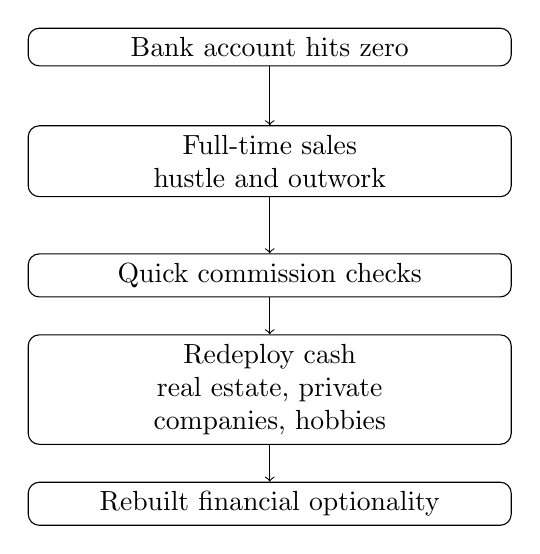
\begin{tikzpicture}[x=1cm,y=1cm]
\node[draw, rounded corners, align=center, text width=5.9cm] (a) at (0,0) {Bank account hits zero};
\node[draw, rounded corners, align=center, text width=5.9cm] (b) at (0,-1.45) {Full-time sales\\ hustle and outwork};
\node[draw, rounded corners, align=center, text width=5.9cm] (c) at (0,-2.9) {Quick commission checks};
\node[draw, rounded corners, align=center, text width=5.9cm] (d) at (0,-4.35) {Redeploy cash\\ real estate, private companies, hobbies};
\node[draw, rounded corners, align=center, text width=5.9cm] (e) at (0,-5.8) {Rebuilt financial optionality};
\draw[->] (a) -- (b);
\draw[->] (b) -- (c);
\draw[->] (c) -- (d);
\draw[->] (d) -- (e);
\end{tikzpicture}
\caption{The rebuilding sequence as Mike gives it: earn first through sales, then redeploy into ownership-like assets.}
\end{figure}

\subsection{Question \& Answer}

\paragraph{Question.}
What survives if the money disappears?

\paragraph{Answer.}
For Mike, the durable asset is not the bank balance. It is the capacity to sell, work, and convert effort into cash flow. Once cash flow returns, the investment menu reopens. In this interview, sales is the first engine because it can be restarted faster than a large balance sheet.

\section{Virtus, Success, and Legacy}

Near the end, the interviewer asks how Mike defines success and how he wants to be remembered. Mike places family first: a happy family life is the foundation. Financial freedom comes next, because it lets a person breathe, pay the bills, leave bad people, get another job, or start something new. A handful of good friends completes the picture.

The legacy answer is consistent with that definition. Mike wants to be remembered as honorable, hard-working, a strong husband and father, authentic and real. He also wants to be remembered as someone who performed forcefully in business. The language is blunt, but the ordering is steady: family foundation first, commercial drive second.

He then describes Virtus. The firm is headquartered in Kansas City, with offices in Fort Collins, Chicago, St. Louis, Austin, Fort Worth, and Memphis. Mike says Virtus has over one hundred people:
\begin{equation}
N_{\text{Virtus people}} > 100.
\end{equation}
He also says the firm has quadrupled in three years:
\begin{equation}
G_{\text{Virtus}} \approx 4
\quad \text{over} \quad
3\ \text{years}.
\end{equation}

The positioning is clear. Mike describes the broader insurance industry as old, slow, and stale; Virtus is presented as young, energetic, specialized, and built for people who want income potential and joy in the job. This closing is not merely a company pitch. It completes the interview's arc: private equity, long-game relationships, specialized sales, family, personal discipline, and legacy all converge in the institution where Mike now spends his energy.

\begin{proposition}
In Mike's account, durable wealth is not only accumulated capital. It is a bundle of cash-flow skill, trusted relationships, specialized knowledge, and personal freedom.
\end{proposition}

\begin{proof}
The transcript supplies the pieces in order. Cash-flow skill appears in the zero-bank-account answer: return to full-time sales and generate commissions. Trusted relationships appear in the long-game story that leads to the later offer. Specialized knowledge appears in the vertical sales teams. Personal freedom appears in Mike's definition of success: the ability to breathe, pay bills, leave bad people, get another job, or start one's own path. The result is not a mathematical theorem, but it is the interview's operating logic.
\end{proof}

\section{Summary}

The interview begins with private equity, but its deeper subject is compounding judgment. Mike's path runs through false starts, a long insurance apprenticeship, high-energy relationships, a private-equity roll-up environment, a move into Virtus, and a later emphasis on coaching and legacy. The main operating lesson is that wealth is not produced by one isolated insight. It is built through rooms, teams, specialties, habits, and cash-flow engines that can be restarted under pressure.

The quantitative anchors are modest but useful: more than two million views on the earlier clip, more than thirty years in insurance, three or four uncertain early years, more than twenty-five years playing the long game, a prior firm of about two thousand people, roughly twenty-five sales people across five or six teams, about ten private-equity specialists, roughly eight hundred restaurant clients, and a firm Mike says quadrupled in three years. For the larger book, Mike's evidence belongs across the durable questions of industry choice, relationships, sales skill, risk recovery, operating discipline, family, legacy, and what wealth is for after the number is reached.